% Figure from MATH 493 notes, section 42 (added, not from lecture). Compile with the notes preamble.
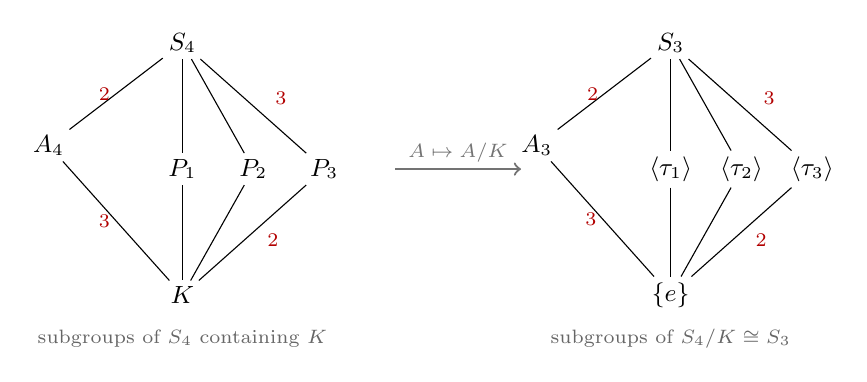
\begin{tikzpicture}[scale=1.0, font=\small, every node/.style={inner sep=2pt}]
\begin{scope}
\node (S) at (0,3.2) {$S_4$};
\node (A) at (-1.7,1.9) {$A_4$};
\node (P1) at (0,1.6) {$P_1$}; \node (P2) at (0.9,1.6) {$P_2$}; \node (P3) at (1.8,1.6) {$P_3$};
\node (K) at (0,0) {$K$};
\draw (S) -- node[left, font=\scriptsize, text=red!70!black] {2} (A);
\foreach \p in {P1,P2,P3} {\draw (S) -- (\p); \draw (\p) -- (K);}
\node[font=\scriptsize, text=red!70!black] at (1.25,2.5) {3};
\node[font=\scriptsize, text=red!70!black] at (1.15,0.7) {2};
\draw (A) -- node[left, font=\scriptsize, text=red!70!black] {3} (K);
\node[font=\scriptsize, text=black!60] at (0,-0.55) {subgroups of $S_4$ containing $K$};
\end{scope}
\draw[->, thick, black!55] (2.7,1.6) -- node[above, font=\scriptsize] {$A \mapsto A/K$} (4.3,1.6);
\begin{scope}[xshift=6.2cm]
\node (S) at (0,3.2) {$S_3$};
\node (A) at (-1.7,1.9) {$A_3$};
\node (P1) at (0,1.6) {$\langle \tau_1 \rangle$}; \node (P2) at (0.9,1.6) {$\langle \tau_2 \rangle$}; \node (P3) at (1.8,1.6) {$\langle \tau_3 \rangle$};
\node (K) at (0,0) {$\{e\}$};
\draw (S) -- node[left, font=\scriptsize, text=red!70!black] {2} (A);
\foreach \p in {P1,P2,P3} {\draw (S) -- (\p); \draw (\p) -- (K);}
\node[font=\scriptsize, text=red!70!black] at (1.25,2.5) {3};
\node[font=\scriptsize, text=red!70!black] at (1.15,0.7) {2};
\draw (A) -- node[left, font=\scriptsize, text=red!70!black] {3} (K);
\node[font=\scriptsize, text=black!60] at (0,-0.55) {subgroups of $S_4/K \cong S_3$};
\end{scope}
\end{tikzpicture}
